\documentclass[a4paper,10pt]{article}

\usepackage{fancyhdr} % clears the header and footer setting
\usepackage{graphicx} 
\usepackage{geometry}
\geometry{a4paper, left=2cm, right=2cm, top=1.5cm, bottom=3cm }
\usepackage{caption}
\usepackage{subcaption}
\usepackage{hyperref}
\usepackage{natbib}
\usepackage{amsmath}


\usepackage{etoolbox,fancyhdr,xcolor}
\newcommand{\headrulecolor}[1]{\patchcmd{\headrule}{\hrule}{\color{#1}\hrule}{}{}}
\newcommand{\footrulecolor}[1]{\patchcmd{\footrule}{\hrule}{\color{#1}\hrule}{}{}}
\renewcommand{\headrulewidth}{1pt}
\headrulecolor{black!100}%
\renewcommand{\footrulewidth}{1pt}
\footrulecolor{red!100}%

\fancyhf{}
\fancyhead[R]{
\includegraphics[width=0.25\textwidth]{figures/nmims.png}}

\fancyfoot[C]{Nilkamal School of Mathematics, Applied Statistics & Analytics}
\fancyfoot[R]{\thepage}

\setlength{\headheight}{15mm}
\pagestyle{fancy} %This command sets the page style to fancy, applying the header and footer configurations defined above to the document pages.

\bibliographystyle{apacite}

\usepackage{times}
\begin{document}

\noindent 
\begin{center}
\textbf{{\Large Movie Recommendation System Using Collaborative Filtering and Content-Based Filtering}} \\
\end{center}

\noindent 
\begin{center}
\textbf{ Zaamena Shamji, Neha Maheshwari, Anushka Jain, Nitya Verma, Aditee Gupta } 
\end{center}\\[-0.5cm]

\begin{center}
\textit{Narsee Monjee Institute Of Management Studies, Mumbai}\\
\end{center}


\noindent 
\begin{center}
    \subsection*{ABSTRACT}
    This project revolves around building a movie recommender system based on conventional techniques like Content-based and drawing up a comparison between them to better understand the implementation of the same by a large number of tech companies. The primary purpose of the project is to build a movie recommender system for new users of an emerging brand in the market.

\end{center}

\noindent 
\textbf{KEYWORDS:} \textit{Collaborative Filtering},\textit{Content-Based Filtering},\textit{Singular Value Decomposition}


\section{INTRODUCTION}

The research objective is to develop and understand the workings and usage of a movie recommendation system. A recommendation system refers to a platform or an engine that provides suggestions for items. The purpose of the recommendation system is to suggest items or products of interest to the users. It studies the relationship between the items and the users to give specific recommendations.

With the increasing growth of content on over-the-top platforms, users often face information load and get overwhelmed. This makes it difficult for the users to choose content that is relevant to their preferences and a one-size-fits-all approach may not be effective. A recommendation system aids diverse users in getting recommendations according to individual tastes and preferences. It helps users narrow down the wide and confusing horizon of options and saves them the time and effort to go through each and every product. This not only helps users get a personalized experience but also assists them in discovering new content that would have been otherwise overlooked due to popular content.

Highly regarded companies like Amazon, Netflix and Spotify use these methods to enhance their customer experience. Their recommendation system utilizes the user's interaction history, their preferences and their similarity with other users to provide recommendations.

For movie recommendations, the project utilizes two types of techniques to provide personalized and relevant suggestions to the users:

\begin{enumerate}
    \item Content-Based Filtering: This method utilizes the past behaviour of the user, to suggest products that are similar to the previously used product of the user. Attributes such as genre, director, actors and generated tags or keywords are analyzed to identify similarities between movies.

    \item Collaborative Filtering: As for collaboration, instead of finding similarities between the items based on the user behaviour, it finds similarities between multiple users and cross-suggests their products to each other. This technique further bisects into two approaches, namely, item-based filtering and user-based filtering.
    \begin{itemize}
        \item Item-based Collaborative Filtering: This focuses on the similarities between the items or the products. Any items sharing similar features are cross-recommended to users who like either of the products.

        \item Model-based Collaborative Filtering:
        This method helps to predict similar movies according to users past interactions as well as other users who are similar to them. This technique requires matrix factorization, which decomposes the user-item interactions to represent latent features.

    \end{itemize}
    
\end{enumerate}

By employing these techniques, the research aims to improve user satisfaction and engagement. This will help the platform to increase viewership and potentially increase revenue.

\section{LITERATURE REVIEW}





\section{DATA}

\subsection{Data Collection}

A secondary research was conducted for this project.  \textbf{Netflix Prize Dataset} and \textbf{Netflix Titles}  datasets were taken into account for building the recommendation system. Both the datasets are available on Kaggle \cite{kaggle}. The "Netflix prize" dataset is the official dataset published by Netflix for an open competition. 

The "Netflix Titles" dataset is an entirely different dataset containing detailed information about each movie.

\subsection{Data Structure}

\textbf{\textit{Netflix Prize Data}} comprises of two text file. The first dataset contains information of the ratings given by the customer to each movie. Table \ref{Data_1} shows the structure of the dataset wherein 

\begin{itemize}
  \item MovieIDs: The unique ID assigned to each movie. It ranges from 1 to 17023 sequentially.
  \item CustomerIDs: The unique ID assigned to each customer. It range from 1 to 2649429, with gaps.
  \item Ratings: Ratings given by each customer. They are on a five-star (integral) scale from 1 to 5.
  \item Dates have the format YYYY-MM-DD.
\end{itemize}
The table shows the ratings given by three different customers to movie Id 1 on the given dates. 






\begin{table}
    \center 
    
    \begin{tabular}{|c|c|c|c|} \hline 
         Customer ID&  Movie ID&  Rating& Date\\ \hline 
         1488844&  1&  3& 2005-09-06
\\ \hline 
         822109&  1&  5& 2005-05-13
\\ \hline 
         885013&  1&  4& 2005-10-19
\\ \hline
    \end{tabular}
    \caption{Customer Rating}   
    \label{Data_1} 
\end{table}

The second dataset contains the titles of the movies corresponding to their respective movie IDs. Table \ref{Movie_titles} shows the structure of the \textit{\textbf{movie titles}} dataset. 

\begin{table}
    \centering
    \begin{tabular}{|c|c|l|} \hline 
         Movie ID& Year Of Release&Title\\ \hline 
         1& 2004&Dinosaur Planet\\ \hline 
         48&  2001&Justice League\\ \hline 
         198
&  1997&Gupt\\ \hline
    \end{tabular}
    \caption{Movie Titles Dataset}
    \label{Movie_titles}
\end{table}

\vspace{10pt}
Figure \ref{netflix titles} shows \textbf{\textit{Netflix Titles}} dataset which contains  information of the movies/Tv shows on Netflix. The dataset contains \textbf{8807} movies in total. The features in the dataset are as follows 
\begin{itemize}
    \item \textbf{Show ID}: Unique ID for every Movie / Tv Show. 
    \item \textbf{Type}:Identifies whether it is A Movie or TV Show 
    \item \textbf{Title} :Title of the Movie / Tv Show 
    \item \textbf{Director}: Director of the Movie
    \item \textbf{Cast}: Actors involved in the movie / show
    \item \textbf{Country}: Country where the movie / show was produced
    \item \textbf{Date} Added: Date it was added on Netflix
    \item \textbf{Release} \textbf{Year}: Actual Release year of the move / show
    \item \textbf{Rating}: TV Rating of the movie / show
    \item \textbf{Duration}:Total Duration - in minutes or number of seasons
    \item \textbf{Listed In}: Genre of the movie/ Show
    \item \textbf{Description}:The summary description 
\end{itemize}
\begin{figure}
    \centering
    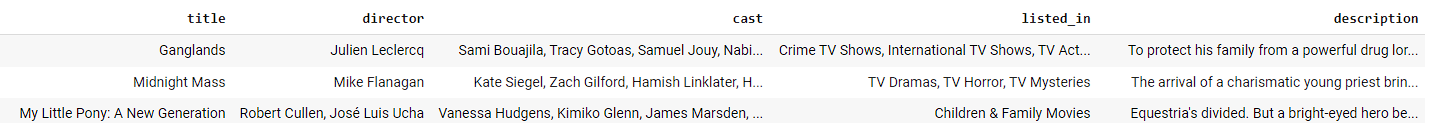
\includegraphics[width=1\linewidth]{figures/netflix_title.png}
    \caption{Netflix Titles Dataset}
    \label{netflix titles}
\end{figure}





\section{Methodology}

\subsection{Data Cleaning}

All the datasets were checked for missing and duplicate values. 
The unnecessary columns like \textit{Date}, \textit{Year Of Release}, \textit{Duration}, etc were deleted. The missing values were either replaced by an empty string, in the case of attributes, or by a zero in the case of numerical columns.  


\subsection{Data Preprocessing}

\subsubsection{Collaborative Filtering}
\textit{\textbf{Netflix Prize dataset}} was used for item-based collaborative filtering. 
\begin{itemize}
    \item \textbf{Merging}: The two datasets (\ref{Data_1} and \ref{Movie_titles}) within the Netflix prize dataset were merged based on the common attribute \textit{MovieID}. The new dataset is given in the figure \ref{Movie_merge}
\end{itemize}

\begin{figure}[ht]
\centering
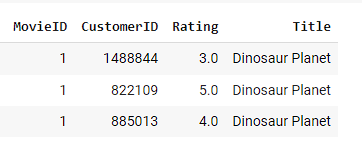
\includegraphics[height=4cm]{figures/movie_data.png}
\caption{Merged Data}
\label{Movie_merge}
\end{figure}


\begin{itemize}
    \item \textbf{Outliers}: The count of ratings given to each movie was calculated. The average count of ratings turned out to be around 26. The outliers were removed by the given formula 
\end{itemize}

\begin{enumerate}
  \item Interquartile Range (IQR):
    \[ \text{IQR} = Q3 - Q1 \]

  \item Upper Limit for Outliers:
    \[ \text{Upper Bound} = Q3 + 1.5 \times \text{IQR} \]
\end{enumerate}

\subsubsection{Content Based Filtering}:

\textbf{\textit{Netflix Titles}} \ref{netflix titles} was used to for content based filtering

\begin{itemize}
    \item \textbf{Stop word removal}: Stopwords are those words which do not add any meaning to the data and are used only to make sense of the information. Words like \textit{a}, \textit{an}, \textit{the}, etc are considered as stopwords. Such words can be removed from the data to increase computational efficiency. 
\end{itemize}


\begin{itemize}
    \item \textbf{Vectorization}: For algorithms to understand textual data, vectorization is used to convert any such data into a numerical value. Vectorization is a natural language processing technique. There are many different methods to perform this process like Bag of Words, TF-IDF, and Word2Vec.We have used Bag of Words to vectorized our data
\end{itemize}

\begin{itemize}
    \item \textbf{Stop word removal}: Stopwords are those words which do not add any meaning to the data and are used only to make sense of the information. Words like \textit{a}, \textit{an}, \textit{the}, etc are considered as stopwords. Such words can be removed from the data so as to increase computational efficiency
\end{itemize}

\begin{itemize}
    \item \textbf{Stemming}: Stemming refers to the process of conversion of words to their base/root form. For example, learn, learning, learned etc have the same meaning, hence they can be converted into their root form that is \textit{learn}. Stemming also helps increase the accuracy and reduces duplication. 
\end{itemize}





\section{Analysis}
\subsection{Collaborative Filtering}

\begin{enumerate}
    \item \textbf{Item-based}: 
    \vspace{2}
    \begin{itemize}
        \item  \textbf{\textit{STEP 1: User Matrix}}
        \vspace{2}
        This step focuses on building the user-movie correlation matrix based on the ratings given by users to all the movies. Figure \ref{user_movie} shows the user-movie matrix 

        \begin{figure}[ht]
        
\centering
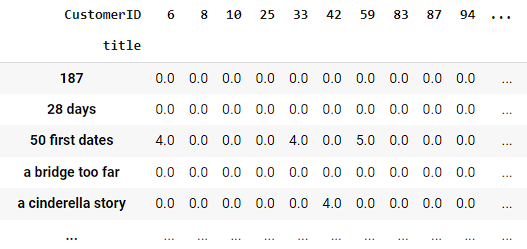
\includegraphics[height=5.5cm]{figures/user_movie.png}
\caption{User Movie Matrix}
\label{user_movie}
\end{figure}
 \item  \textbf{\textit{STEP 2: Similarity Score }} 
        Similarity score is calculated between the items to find the likeness in item characteristics. The items in a movie recommendation system are the movies and hence the similarity score is calculated to find out the extent of similarity between all the movies.

        The formula for cosine similarity between two vectors
The formula for cosine similarity between two vectors $\mathbf{A}$ and $\mathbf{B}$ is given by:

\[
\text{Cosine Similarity}(\mathbf{A}, \mathbf{B}) = \frac{\mathbf{A} \cdot \mathbf{B}}{\|\mathbf{A}\| \cdot \|\mathbf{B}\|}
\]


If the similarity score is closer to 0 it indicates poor similarity among items and a score closer to 1 indicates a stronger similarity among items. After calculating the similarity score using the above formula, the next step is to build the similarity matrix. 
The items are most similar to each other hence the similarity matrix forms a correlation matrix with diagonal elements as 1.

Following figure \ref{similarity(item)} is a part of the similarity matrix of the dataset:

    \begin{figure}[ht]
        
        \centering
        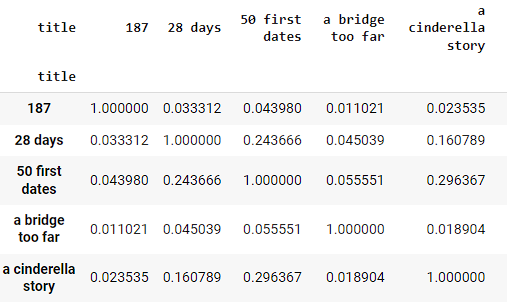
\includegraphics[height=5.5cm]{figures/similarity(item).png}
        \caption{Similarity matrix}
        \label{similarity(item)}
\end{figure}

\item \textbf{\textit{STEP 4: Recommendation Function}}
This is the last step which is based on building the recommendation system. Before proceeding with the construction of the function, the similarity scores are standardized and normalized by multiplying the similarity score of the movies with the standardized ratings. The ratings are standardized by subtracting the mean of the ratings which is 2.5.

Further, the standardized ratings are sorted and arranged so that the most similar movies are recommended. Given below \ref{recommend(item)} are the recommendations of the movie \textit{Jaws} with the corresponding similarity scores
\begin{figure}[ht]
        
        \centering
        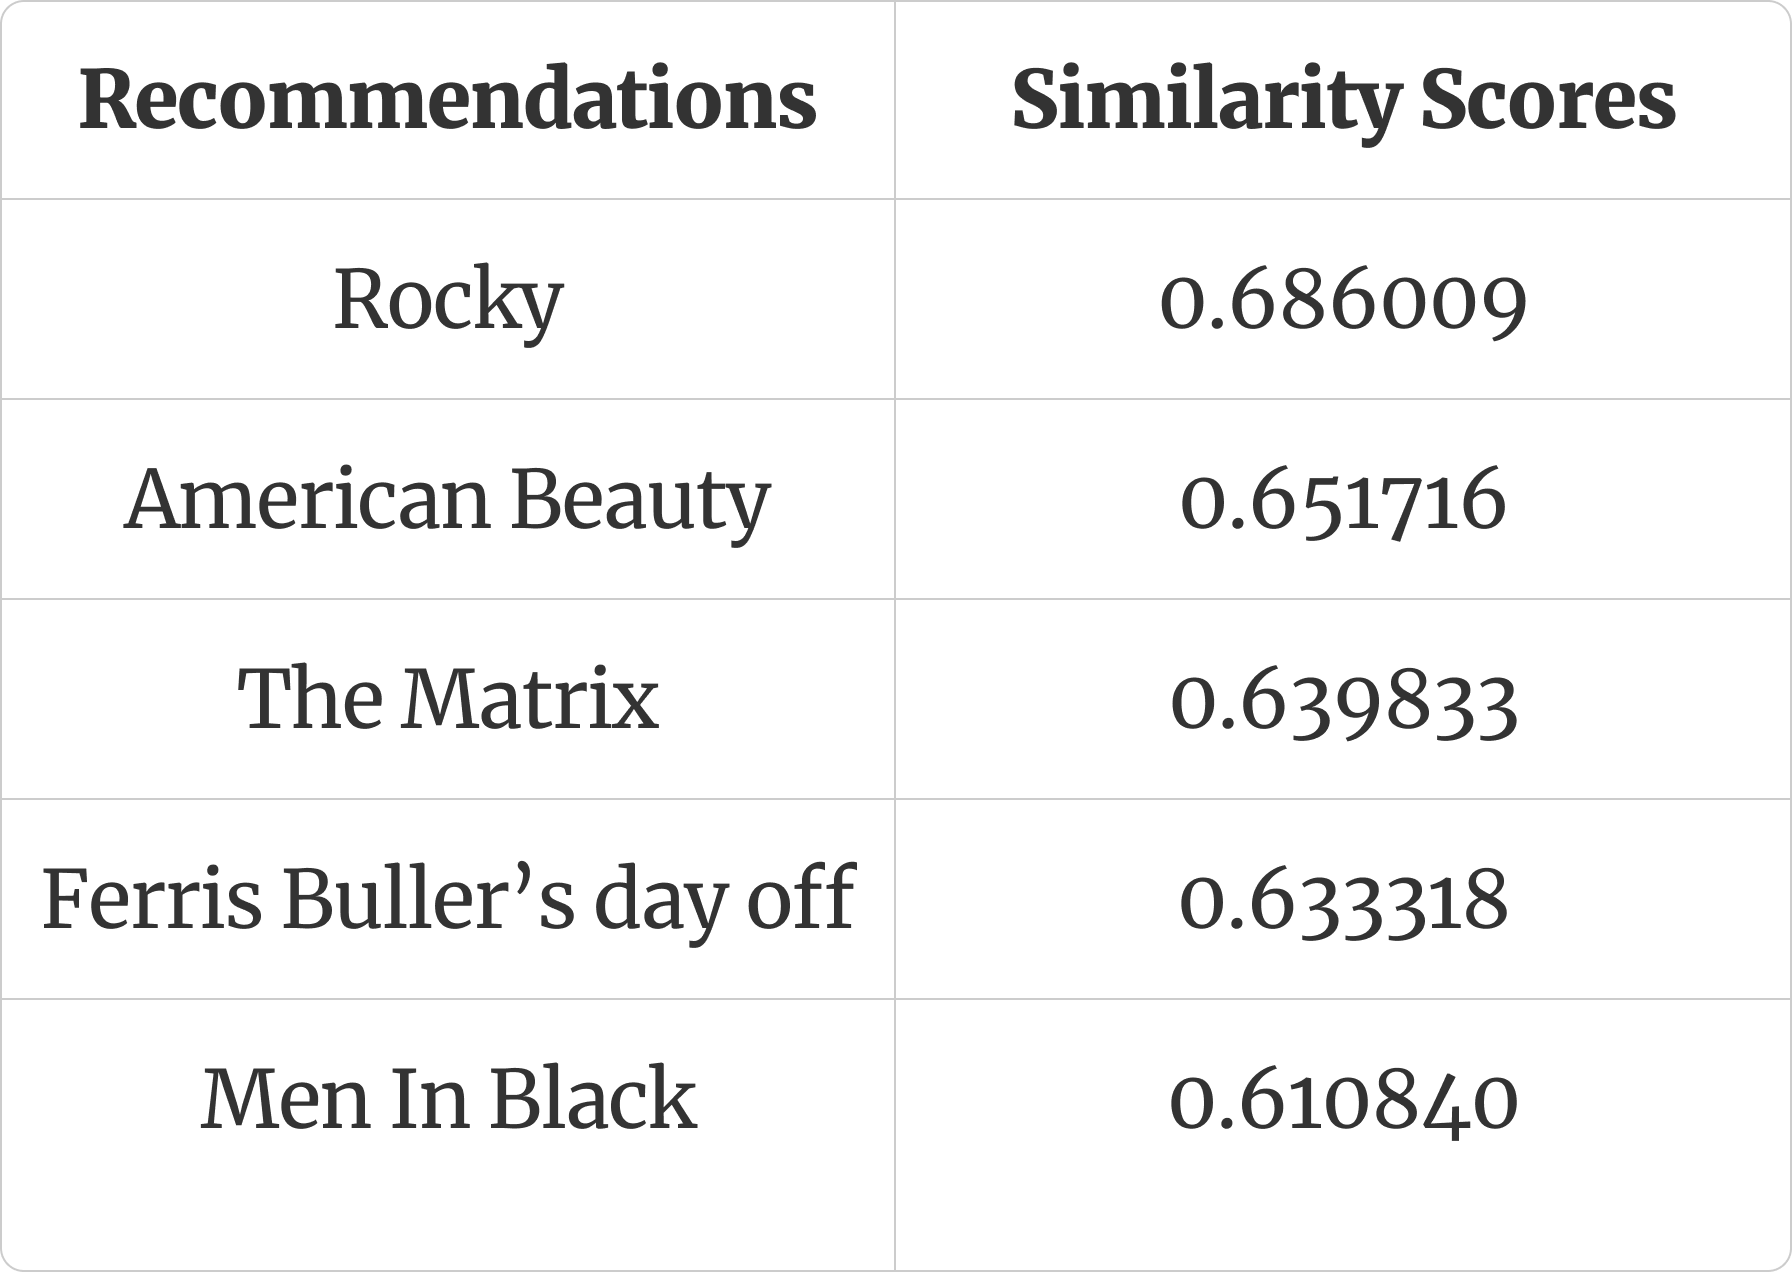
\includegraphics[height=4.3cm]{figures/recommend(item).png}
        \caption{Recommendations of the movie with similarity score}
        \label{recommend(item)}
\end{figure}

The function is so built that if any movies are not a part of the dataset then the most rated movies are recommended instead

\begin{figure}[ht]
        
        \centering
        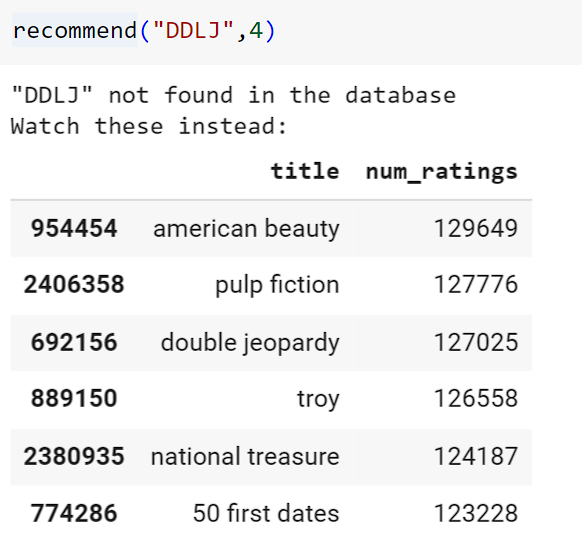
\includegraphics[height=6.6cm]{figures/not_in_db.png}
        \caption{Movie not found in the database}
        \label{not in db}
\end{figure}
    \end{itemize}


\item \textbf{Singular Value Decomposition:}: 
    \vspace{2}
\end{enumerate}


\subsection{Content-Based Filtering}
\begin{itemize}
    \item  \textbf{\textit{STEP 1: Create Tags}} 
    From the \textit{Netflix Titles} dataset, we will  create tags by combining the relevant columns. \textit{Description}, \textit{Listed in (genre)}, \textit{Cast}, \textit{Director} of each movie were merged in order to create the tags. The data frame \ref{tags} shows the created tags


\begin{figure}[ht]
        
        \centering
        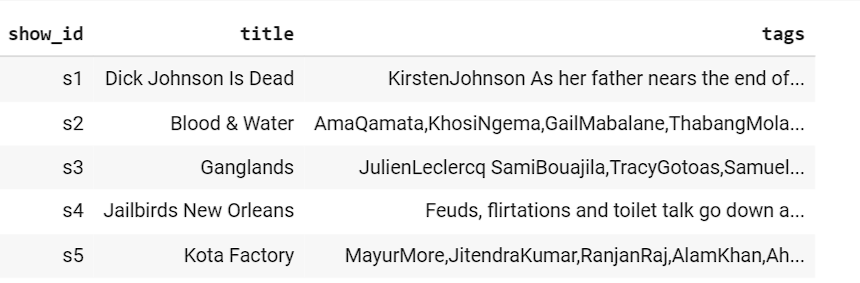
\includegraphics[height=5cm]{figures/tags.png}
        \caption{Dataframe containing tags of each movie}
        \label{tags}
\end{figure}

    \item  \textbf{\textit{STEP 2: Vectorization}}
    The next step is vectorization by the ‘Bag of words’ algorithm. This feature is used as an extraction technique that models text data for processing in information retrieval. This technique is applied to the previously created tags to numerical data for further processing.

    \item  \textbf{\textit{STEP 3: Similarity Scores}}
    The similarity score is calculated between the items to find the likeness in item characteristics. The items in a movie recommendation system are the movies and hence the similarity score is calculated to find out the extent of similarity between all the movies based on features like cast, description, title, director etc.

    \item  \textbf{\textit{STEP 4: Recommendation Function}}
    The last step aims at building the recommendation system based on the similarity score of the movies. The movie with the highest similarity score is recommended. The function is so built that if any movies are not a part of the dataset then the most rated movies are recommended instead.

\begin{figure}[ht]
        
        \centering
        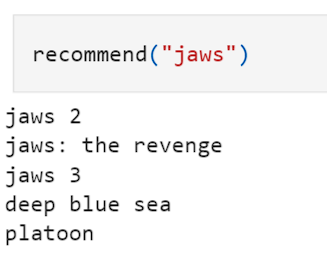
\includegraphics[height=4.3cm]{figures/recommend(content).png}
        \caption{Recommendations using Content-Based Filtering}
        \label{recommend(content)}
\end{figure}


\end{itemize}

\section{CONCLUSIONS}

\section{LIMITATIONS}
\begin{itemize}
    \item Geographic limitations in the data.
    \item Cold start problem: Item-based recommendation highly depends on the user’s past data therefore, the model cannot be used for new users.

    \item If a user doesn't have enough similar users, predicting accurate recommendations would be a problem.
\end{itemize}


\section{FUTURE SCOPE}
\begin{itemize}
    \item The hybrid technique which combines the two models can be used to get more accurate results.
    \item Context-based collaborative filtering can also be merged to geographically and culturally distribute the data.
    \item Development of real-time machine learning and deep learning models.
\end{itemize}
\fontsize{8}{9}\selectfont
\bibliography{ResearchPaperBib}



\clearpage



\end{document}